The scattering of two positively charged W bosons is proceeding at the LHC through the partonic process:
%
\begin{equation}
\Pp\Pp\to\mu^+\nu_\mu{\rm e}^+\nu_{\rm e}\,\Pj\Pj+\mathrm{X}.
\end{equation}

This process possesses three LO contributions of different orders.
The first one is of order $\mathcal{O}{\left(\alpha^{6}\right)}$ and is referred to as EW contribution.
In addition to typical VBS contributions, as shown on the left of Fig.~\ref{diag:LO}, it also features $s$-channel contributions.
Note that we define $s$-, $t$-, and $u$-channel contributions by looking at the process which is contained by only looking at the quark lines.
The $s$-channels will play a particular role in the study of the various contributions in Sec.~\ref{subsec:contributions}.
Some of them take the form of decay chains, for example the diagram represented in the middle of Fig.~\ref{diag:LO}, while others are tri-boson contributions (right of Fig.~\ref{diag:LO}).
The VBS diagrams typically dominate the full process.
But all these contributions form a single gauge-invariant set of contributions and therefore cannot be separated.

The process can also be mediated via a gluon connecting the two quark lines while the W bosons are radiated off the quark lines.
These contributions are of order $\mathcal{O}{\left(\alphas^{2}\alpha^{4}\right)}$ and feature different kinematical behaviours than the EW contribution.
Nonetheless they share the same final state and therefore constitute an irreducible background.

Finally, due to the specific colour structure of these two classes of amplitudes, there exist non-zero interferences if only one quark family is involved.
These are of order $\mathcal{O}{\left(\alpha_{\rm s}\alpha^{5}\right)}$ and are usually small but not negligible for realistic experimental set-ups \cite{Biedermann:2017bss}.

In experimental measurements, special VBS-cuts are designed to enhance the EW contribution over the QCD one.
These cuts are based on the fact that the two contributions have different kinematical behaviour.
The EW contribution is characterised by two jets with large rapidities as well as a large invariant mass.
The two W bosons are mostly produced centrally.
This is in contrast to the QCD contribution which favours jets in the central region.
Therefore, the event selection usually involves rapidity-difference and invariance-mass cuts for the jets.
This will also be discussed in Sec.~\ref{subsec:contributions}.

\begin{figure*}[t]
\begin{center}
          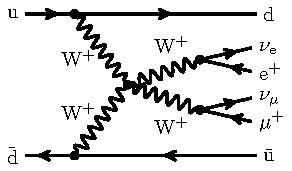
\includegraphics[width=0.30\linewidth]{feynman/LO_EW_5}
          \raisebox{.5ex}{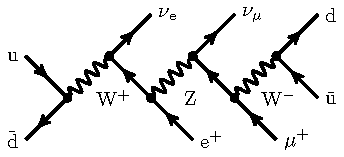
\includegraphics[width=0.35\linewidth]{feynman/LO_EW_2}}
          \raisebox{-1.8ex}{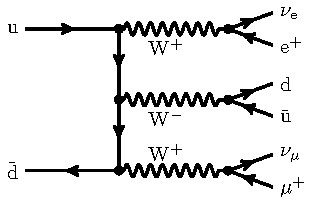
\includegraphics[width=0.32\linewidth]{feynman/LO_EW_3}}
\end{center}
        \caption{Sample tree-level diagrams that contribute to the process $\Pp\Pp\to\mu^+\nu_\mu\Pe^+\nu_{\Pe}\Pj\Pj$ at order $\mathcal{O}{\left(\alpha^{6}\right)}$.
        In addition to typical VBS contribution (left), this order also possesses $s$-channel (middle) and tri-boson contributions (right). }
\label{diag:LO}
\end{figure*}
